\section{Lenguajes nativos}

\begin{frame}[t]{Programa nativo}
  \begin{itemize}
    \item Un \textbf{programa nativo} es un programa de computador que se ejecuta directamente en el juego de instrucciones de la máquina.
      \begin{itemize}
        \item Contiene instrucciones de la ISA sobre la que se ejecuta.
        \item No requiere ninguna traducción durante su ejecución.
        \item Puede contener llamadas a un sistema operativo concreto.
      \end{itemize}
  \end{itemize}
\end{frame}

\begin{frame}[t]{Ensamblador}
  \begin{itemize}
    \item Decada de los 40:
      \begin{itemize}
        \item Programas en código máquina codificados directamente comos secuencia de valores binarios.
        \item Aparece la idea de ensamblador.
      \end{itemize}
  \end{itemize}
  \pause
\begin{columns}
  \begin{column}{0.2\textwidth}
    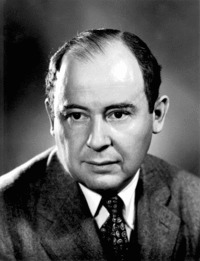
\includegraphics[width=.8\textwidth]{images/von-neumann.jpg}
  \end{column}
  \begin{column}{0.8\textwidth}
    \begin{quote}
      Why would you want more than machine language?
    \end{quote}
    John von Neumann (1903-1957)
  \end{column}
\end{columns}
\pause
\begin{itemize}
  \item Aparecen lenguajes ensambladores y herramientas asociadas:
    \begin{itemize}
      \item Ensamblador (assembler): Traduce a código objeto.
      \item Editor de enlaces (linker): Fusiona módulos de código objeto en un ejecutable en código máquina.
    \end{itemize}
\end{itemize}
\end{frame}

\begin{frame}[t]{Problemas con el ensamblador}
  \begin{itemize}
    \item Dificultad:
      \begin{itemize}
        \item Muy conducente a errores.
      \end{itemize}
    \item Portabilidad:
      \begin{itemize}
        \item Lenguaje específico para cada arquitectura de procesador.
      \end{itemize}
    \item Escalabilidad:
      \begin{itemize}
        \item Limita el tamaño de los productos software al no permitir dominar la complejidad.
      \end{itemize}
  \end{itemize}
\end{frame}

\begin{frame}[t]{Lenguajes de programación}
  \begin{itemize}
    \item \textbf{\color{blue}Plankalk\"{u}l}
      \begin{itemize}
        \item 1943-1945: Konrad Zuse.
        \item No implementado hasta 1998.
      \end{itemize}
    \pause
    \item \textbf{\color{blue}Short Code}
      \begin{itemize}
        \item 1949: Representación de expresiones matemáticas en forma comprensible.
        \item Código traducido a código máquina cada vez que se ejecuta.
      \end{itemize}
    \pause
    \item \textbf{\color{blue}Autocode}
      \begin{itemize}
        \item 1952: Primer lenguaje compilado.
      \end{itemize}
    \pause
    \item Lenguajes de dominio específico:
      \begin{itemize}
        \item 1954: Fortran.
        \item 1959: COBOL.
      \end{itemize}
  \end{itemize}
\end{frame}

\begin{frame}[t]{Algunos paradigmas fundamentales}
  \begin{itemize}
    \item \textbf{\color{blue}Simula}: Programación orientada a objetos.
      \begin{itemize}
        \item Compilado.
      \end{itemize}
    \item \textbf{\color{blue}C}: Programación de sistemas portable.
      \begin{itemize}
        \item Compilado.
      \end{itemize}
    \item \textbf{\color{blue}Prolog}: Programación lógica.
      \begin{itemize}
        \item Compilado a código máquina abstracto.
      \end{itemize}
    \item \textbf{\color{blue}Lisp}: Programación funcional.
      \begin{itemize}
        \item Interpretado.
      \end{itemize}
    \item \textbf{\color{blue}ML}: Progrmación funcional fuertemente tipada con polimorfismo.
      \begin{itemize}
        \item Interpretado.
      \end{itemize}
  \end{itemize}
\end{frame}

